Our program is divided in two main modules, the mapping module and the planning module.
The role of the first one is to build the map of the environment of the robot using the echoes of the lasers.
The role of the second one is to plan the path that the robot must follow in order to explore the world.

To communicate with the MRDS server we created a class named 'Robot', it is used as an interface to send and receive informations to and from the MRDS server easily.
The received informations are directly adapted to our needs and stored using our 'Position' and 'Laser' datastructures in this class.

\section{Mapping}

The first point on which we worked was to find a way of building a map of the environment of the robot using the lasers echoes.

To do so we created a class 'Map' that contains a grid of values between $0$ and $1$.
Those values represent probability that there is an obstacle on that cell.
All the values are initialized to $0.5$ which is the average value between $0$ and $1$ since we do not know if there is an obstacle or not at that place.

To update this grid we created a class 'Cartographer' that uses the echoes of the lasers.
For each laser echoe we compute the distance between the robot cell and the cell hit by the laser in the grid.
Then we use the 'Bresenham' algorithm to update all the cells in between the two above.
For all those cells we compute an increment that is added or subtracted to them using the following procedure:

\begin{enumerate}
    \item First we compute an increment factor in regard of the value of the cell:
        $$
        inc\_factor\_iro\_certainty = 1 - (abs(cell_value - 0.5) \cdot 2)
        $$
    \item Then we compute an increment factor in regard of the distance between the robot and the cell to update:
        $$
        inc\_factor\_iro\_dist = 1.5 \cdot (1 - abs(distance / max\_lasers\_distance))
        $$
    \item The final increment is computed by multiplying the two factors with a defined increment value (we used 0.1):
        $$
        final\_increment = inc\_factor\_iro\_certainty \cdot inc\_factor\_iro\_dist \cdot increment
        $$
    \item The final increment is added to the cell if the cell corresponds to the cell hit by the laser and that the distance of the echoe is below the maximum laser distance.
        Otherwise it is subtracted.
\end{enumerate}

The certainty factor is useful because it will make the cells that are near $0$ and near $1$ harder to change than the cells near $0.5$, the effect is that the cells defined as obstacle will have to be seen as empty for a long time before being changed and inversely.
The distance factor is useful because it will make the cells near the robot update more easily than the cells far away, since the further away the cell is from the robot the less precise the laser information is.

This is the factory map built moving the robot by hand using the cartographer described above.

\FloatBarrier
\begin{figure}
    \centering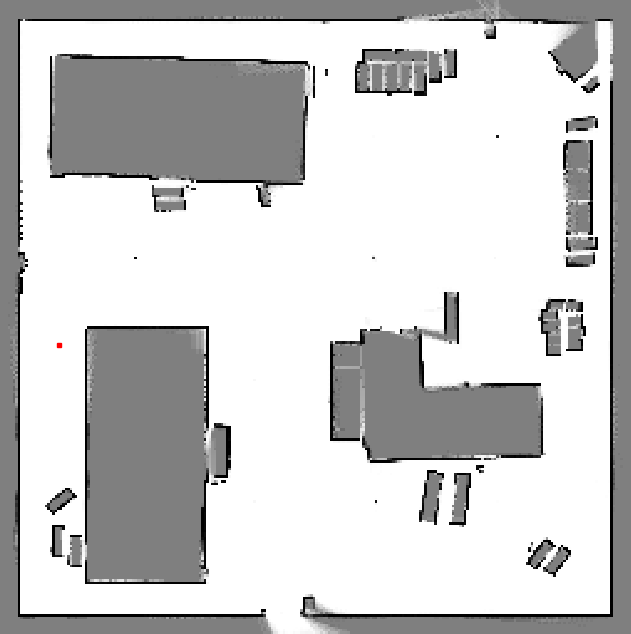
\includegraphics[width=\textwidth]{explored_map_by_hand.png}
    \label{fig:explored_map_by_hand}
    \caption{Explored map by hand}
\end{figure}
\FloatBarrier

The mapping module also contains the 'ShowMap' class which is used to display the built map.

\section{Planning}

TODO

